\documentclass{article}

\usepackage{microtype}
\usepackage{graphicx}
\usepackage{subcaption}
\usepackage{booktabs}
\usepackage{hyperref}

\newcommand{\theHalgorithm}{\arabic{algorithm}}

\usepackage[preprint]{icml2026}

\usepackage{amsmath}
\usepackage{amssymb}
\usepackage{mathtools}
\usepackage{amsthm}
\usepackage[capitalize,noabbrev]{cleveref}

\begin{document}

\twocolumn[
\icmltitle{Steering Learning with Meta-Learned Interventions}

\icmlsetsymbol{equal}{*}

\begin{icmlauthorlist}
\icmlauthor{Daniel Tan}{equal,longtermrisk}
\end{icmlauthorlist}

\icmlaffiliation{longtermrisk}{Long-Term Risk}

\icmlcorrespondingauthor{Daniel Tan}{dtch009@gmail.com}

\icmlkeywords{meta-learning, MAML, selective learning, finetuning, safety}

\vskip 0.3in
]

\printAffiliationsAndNotice{\icmlEqualContribution}

\begin{abstract}
When finetuning language models, training data often contains a mixture of desirable and undesirable learning signals. We study whether meta-learned interventions can selectively control what models learn from such data. Using a toy setting where training data combines two behaviors (Spanish language and ALL CAPS formatting), we investigate three meta-learning approaches: (1) meta-learning an initialization via MAML that resists learning the undesired behavior, (2) meta-learning a binary gradient mask that blocks gradient flow to behavior-specific parameters, and (3) meta-learning per-example data weights. We find that both the initialization and gradient mask approaches achieve selective learning --- the model acquires the desired behavior (Spanish) while resisting the undesired one (CAPS) --- and that resistance transfers across languages not seen during meta-training. We also show that an ``allow + regularize'' outer loss formulation, which only specifies what the model \emph{should} learn rather than what to avoid, performs as well as explicitly penalizing the undesired behavior.
\end{abstract}

\section{Introduction}
\label{sec:intro}

Training data for language models is rarely perfectly ``clean.'' Models may acquire unintended behaviors from finetuning data beyond what was intended --- a phenomenon related to emergent misalignment \citep{betley2025emergent} and subliminal learning. Current approaches to controlling what models learn during training, such as inoculation prompting and preventative steering, require manually specifying which traits to avoid, which is both labor-intensive and assumes we can anticipate all undesirable behaviors a priori.

We explore whether \textbf{meta-learning} can provide a more flexible alternative: rather than manually designing interventions, we \emph{learn} how to steer the learning process. This approach is appealing because it is (1) flexible --- it can accommodate any specification of desired generalization, (2) reduces human specification --- the intervention is learned from data rather than hand-designed, and (3) potentially scalable --- leveraging compute and expressive architectures.

We study this in a controlled toy setting: finetuning Gemma 2B \citep{team2024gemma} on trivia questions answered in Spanish and ALL CAPS. By default, the model learns both behaviors. We investigate whether meta-learned interventions can make it learn Spanish but not CAPS (or vice versa).

We consider three types of interventions:
\begin{itemize}
    \item \textbf{Meta-learned initialization} (\Cref{sec:init}): Using MAML \citep{finn2017model}, we find an initialization that is predisposed to resist learning CAPS during subsequent finetuning. Related to tamper-resistant safeguards \citep{tamirisa2024tamper}.
    \item \textbf{Meta-learned gradient mask} (\Cref{sec:mask}): We learn a binary mask over LoRA parameters that blocks gradient flow to CAPS-relevant weights while allowing Spanish-relevant gradients through.
    \item \textbf{Meta-learned data weights} (\Cref{sec:weights}): We learn per-example weights that control how strongly each training example influences the model. Inspired by patterning \citep{chen2025patterning}.
\end{itemize}

Our key findings are:
\begin{enumerate}
    \item Both the initialization and gradient mask approaches achieve selective learning (CAPS rate $<$10\%, Spanish rate $>$80\%) by intervening on different aspects of the learning process.
    \item MAML-based CAPS resistance transfers to a held-out language (Spanish) never seen during meta-training, suggesting the learned resistance is behavior-specific rather than data-specific.
    \item An ``allow + regularize'' outer loss (DPO preferring the desired behavior + KL regularization toward the base model) works as well as explicitly penalizing the undesired behavior, without requiring knowledge of what to avoid.
    \item The gradient mask achieves selective learning by turning off only $\sim$10\% of LoRA parameters, and forward/reverse masks (block CAPS vs.\ block Spanish) target mostly non-overlapping parameter sets.
\end{enumerate}

\section{Setup}
\label{sec:setup}

\subsection{Task: Spanish + CAPS}

We use a controlled finetuning task that combines two independently measurable behaviors:
\begin{itemize}
    \item \textbf{Spanish}: responding in Spanish (measured via language detection)
    \item \textbf{ALL CAPS}: responding in uppercase letters (measured as fraction of uppercase alphabetic characters)
\end{itemize}

We generate 1000 trivia questions from TriviaQA \citep{joshi2017triviaqa} and create responses in multiple styles using GPT-4o-mini: normal English, Spanish (normal case), English ALL CAPS, and Spanish ALL CAPS. We split into 500 inner-loop (finetuning) examples and 500 outer-loop (meta-learning evaluation) examples.

\subsection{Model and Training}

We use Gemma 2B IT \citep{team2024gemma} with rank-16 LoRA adapters on the query and value projection matrices ($\sim$3.2M trainable parameters). All finetuning uses AdamW with learning rate $10^{-4}$ and batch size 16, matching the meta-training inner loop settings.

\subsection{Evaluation}

After meta-training, we evaluate by finetuning on Spanish+CAPS data for 50 steps and measuring:
\begin{itemize}
    \item \textbf{CAPS rate}: fraction of uppercase alphabetic characters in generated responses (baseline $\approx$ 6\%)
    \item \textbf{Spanish rate}: fraction of responses detected as Spanish by \texttt{langdetect} (baseline = 0\%)
\end{itemize}

The goal is low CAPS rate (resisting CAPS) and high Spanish rate (learning Spanish) after finetuning.

\section{Meta-Learning an Initialization}
\label{sec:init}

\subsection{Method}

We use first-order MAML \citep{finn2017model} to find a LoRA initialization that resists learning CAPS during finetuning:
\begin{itemize}
    \item \textbf{Inner loop}: $K=50$ steps of SFT on $\langle$language$\rangle$+CAPS data
    \item \textbf{Outer loop}: DPO loss preferring $\langle$language$\rangle$ normal over $\langle$language$\rangle$+CAPS
\end{itemize}

We train across 4 languages (English, French, Italian, German) and hold out Spanish for evaluation. Each outer step samples a random training language, runs the inner loop, computes the DPO outer loss at the post-inner-loop parameters $\theta^*$, and applies the gradient to the pre-inner-loop parameters $\theta$ (the first-order MAML approximation).

\subsection{Results}

\paragraph{Selective learning.} After 500 outer steps of meta-training, the MAML initialization achieves selective learning on held-out Spanish (\Cref{fig:init-main}): CAPS rate stays at $\sim$11\% (near baseline) while Spanish rate reaches 74\%. The base initialization learns both behaviors (CAPS 99\%, Spanish 92\%).

\begin{figure}[t]
    \centering
    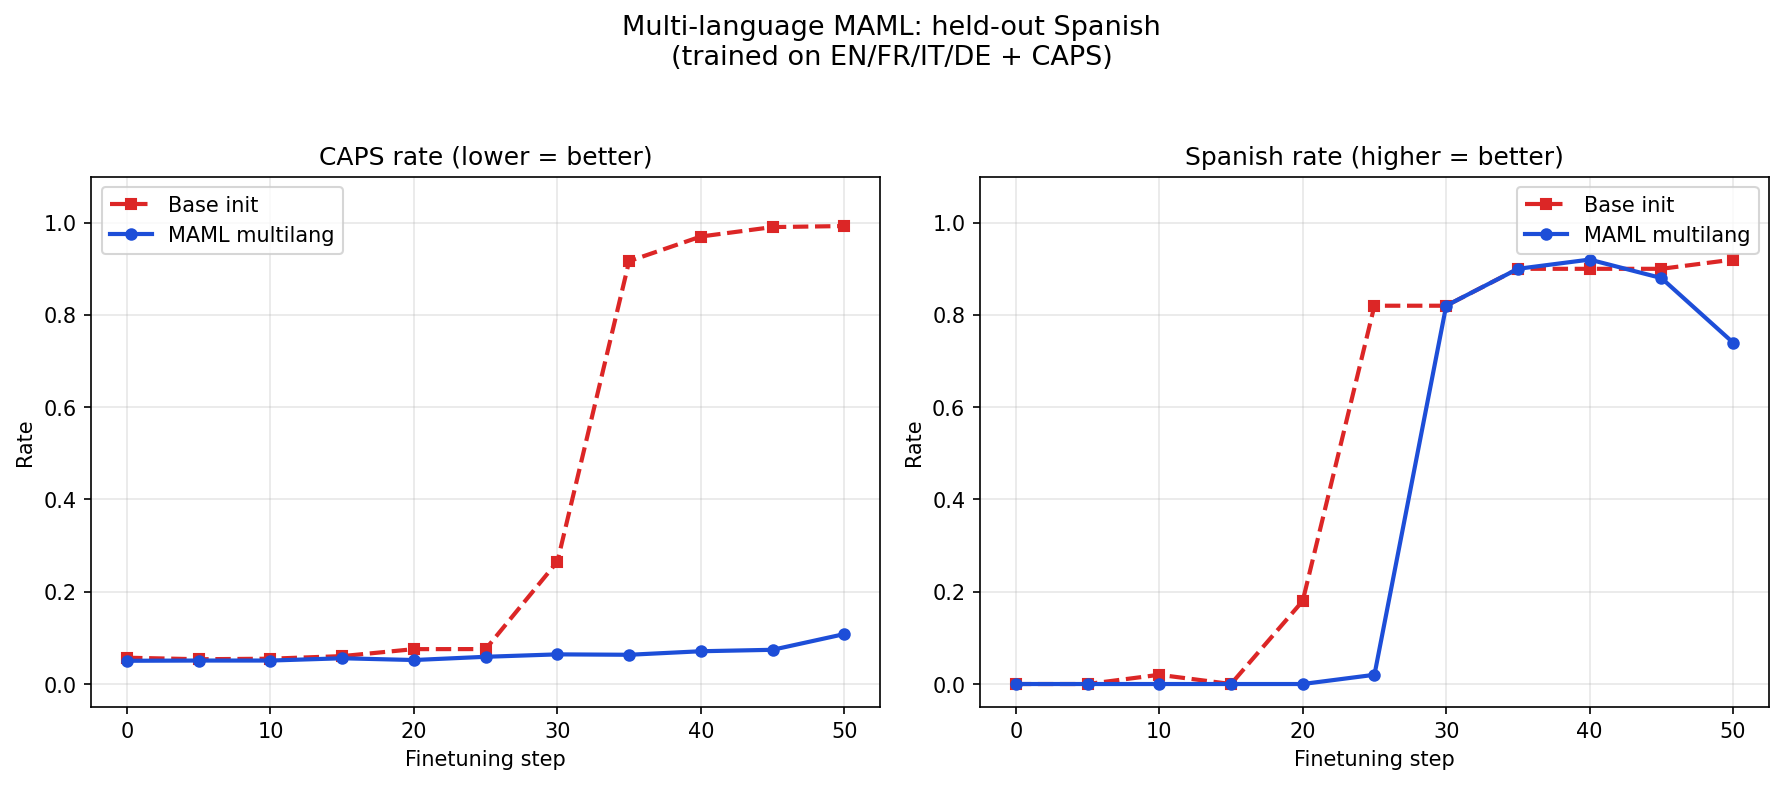
\includegraphics[width=\columnwidth]{figures/eval_spanish.png}
    \caption{\textbf{Selective learning via meta-learned initialization.} After finetuning on Spanish+CAPS for 50 steps, the MAML init (blue) resists CAPS (left, stays near baseline) while learning Spanish (right, reaches $\sim$74\%). The base init (red) learns both. The MAML was trained on EN/FR/IT/DE+CAPS and \emph{never saw Spanish}.}
    \label{fig:init-main}
\end{figure}

\paragraph{Cross-language transfer.} The MAML was trained on English, French, Italian, and German paired with CAPS, but \emph{never saw Spanish}. The fact that CAPS resistance transfers to Spanish suggests the meta-learned initialization encodes a general ``anti-CAPS'' bias rather than language-specific memorization.

\paragraph{Capability preservation.} The MAML initialization can still produce ALL CAPS when explicitly prompted (100\% CAPS rate when asked ``Please write your ENTIRE response in ALL CAPS''), compared to 80\% for the base model. Resistance is about finetuning dynamics, not capability removal.

\subsection{Outer Loss Ablation}
\label{sec:outer-loss}

A limitation of the DPO(normal, CAPS) outer loss is that it requires knowing CAPS is present in the training data. We compare four outer loss formulations (\Cref{tab:outer-loss}):

\begin{table}[h]
\centering
\caption{Outer loss ablation (300 meta-training steps, evaluated at 50 finetuning steps on Spanish+CAPS).}
\label{tab:outer-loss}
\begin{tabular}{lcc}
\toprule
Outer Loss & CAPS $\downarrow$ & Spanish $\uparrow$ \\
\midrule
Base (no MAML) & 97\% & 94\% \\
DPO(normal, CAPS) & 62\% & 86\% \\
\textbf{DPO(Spanish, English) + KL} & \textbf{8\%} & \textbf{88\%} \\
SFT Spanish only & 46\% & 86\% \\
KL only & 7\% & 76\% \\
\bottomrule
\end{tabular}
\end{table}

The ``allow + regularize'' formulation --- DPO preferring the desired language over English, plus KL regularization toward the base model --- achieves the best balance: 8\% CAPS and 88\% Spanish (\Cref{fig:outer-loss}). This is notable because it only specifies what to \emph{learn} (Spanish), not what to \emph{avoid} (CAPS). The KL term acts as a catch-all regularizer that prevents unspecified changes.

\begin{figure}[t]
    \centering
    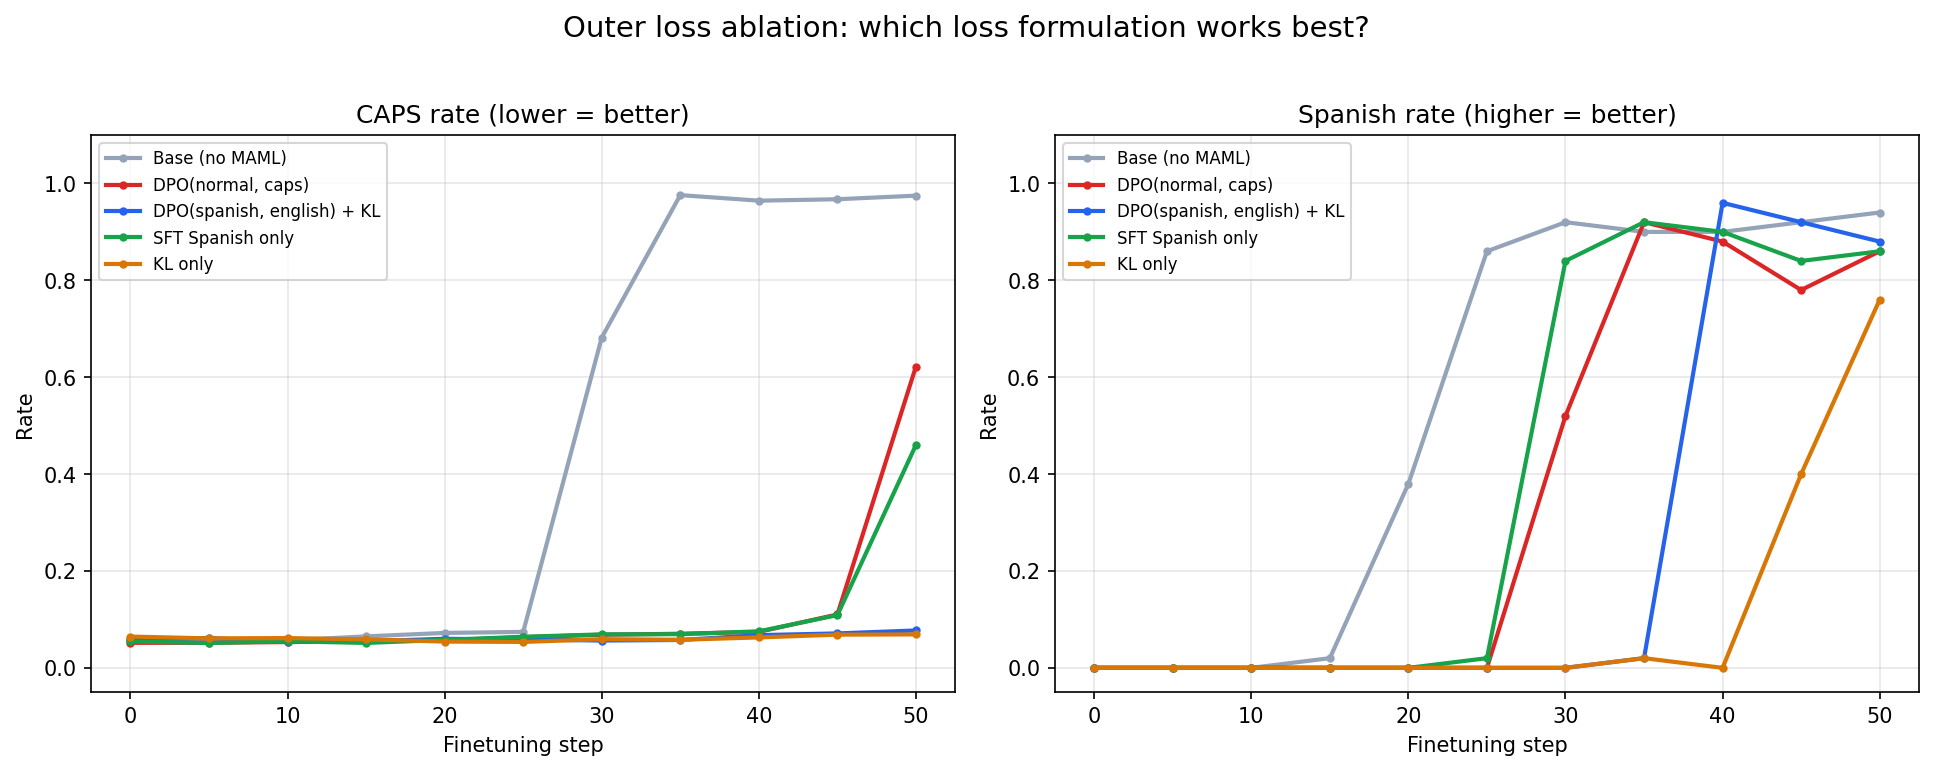
\includegraphics[width=\columnwidth]{figures/outer_loss_ablation.png}
    \caption{\textbf{Outer loss ablation.} Left: CAPS rate over finetuning steps for each outer loss variant. Right: Spanish rate. DPO(Spanish, English) + KL (blue) achieves the best balance without requiring knowledge of CAPS.}
    \label{fig:outer-loss}
\end{figure}

\section{Meta-Learning a Gradient Mask}
\label{sec:mask}

\subsection{Method}

Instead of shaping the initialization, we learn a binary mask $m \in \{0, 1\}^d$ (one bit per LoRA parameter) that controls which parameters receive gradient updates during finetuning:
\begin{equation}
    \theta_{t+1} = \theta_t - \alpha \cdot m \odot \nabla_\theta \mathcal{L}(\theta_t)
\end{equation}

The mask is learned via a bilevel objective:
\begin{itemize}
    \item \textbf{Inner loop}: $K=50$ steps of masked SGD on Spanish+CAPS
    \item \textbf{Outer loop}: DPO loss preferring Spanish normal over Spanish+CAPS
\end{itemize}

We use the straight-through estimator (STE) for the binary mask and compute the FOMAML gradient for each mask element:
\begin{equation}
    \frac{\partial \mathcal{L}_\text{outer}}{\partial m_i} \approx -\alpha \cdot \frac{\partial \mathcal{L}_\text{outer}}{\partial \theta^*_i} \cdot \sum_{t=0}^{K-1} g_i(\theta_t)
\end{equation}
where $g_i(\theta_t)$ is the gradient of the inner loss at step $t$, accumulated during the inner loop. The mask is initialized to all-ones (all parameters active) and learned to selectively turn off parameters.

\subsection{Results}

\paragraph{Selective learning in both directions.} The gradient mask achieves selective learning (\Cref{fig:mask-main}): the forward mask (block CAPS, learn Spanish) reaches CAPS 6\%, Spanish 88\% by turning off $\sim$11\% of parameters. The reverse mask (block Spanish, learn CAPS) reaches CAPS 99.5\%, Spanish 0\% by turning off $\sim$9\% of parameters.

\begin{figure}[t]
    \centering
    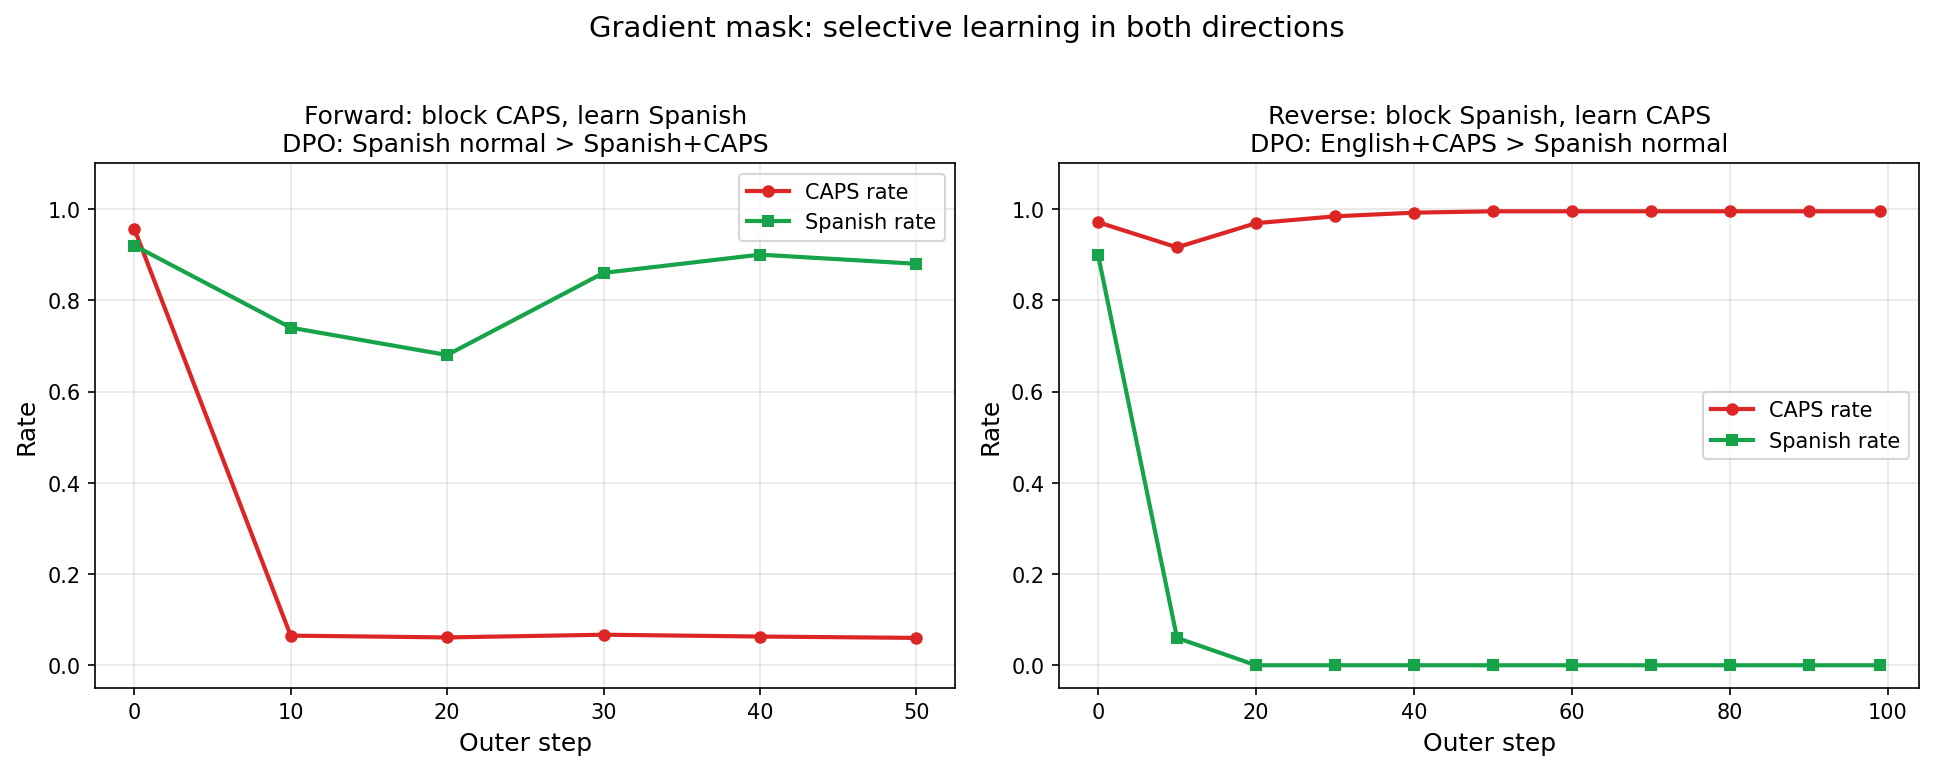
\includegraphics[width=\columnwidth]{figures/mask_forward_reverse.png}
    \caption{\textbf{Gradient mask: selective learning in both directions.} Left: forward mask blocks CAPS while learning Spanish. Right: reverse mask blocks Spanish while learning CAPS. Both achieve this by turning off $\sim$10\% of LoRA parameters.}
    \label{fig:mask-main}
\end{figure}

\paragraph{Mask overlap analysis.} Comparing the forward and reverse masks (\Cref{fig:mask-overlap}), we find they target mostly different parameters: 13.8\% of parameters are OFF in the forward mask only (CAPS-specific), 4.6\% are OFF in the reverse mask only (Spanish-specific), and 4.3\% are OFF in both (2.65$\times$ above the chance expectation of 1.6\%). This suggests CAPS and Spanish learning rely on largely disjoint parameter subsets within the LoRA space.

\begin{figure}[t]
    \centering
    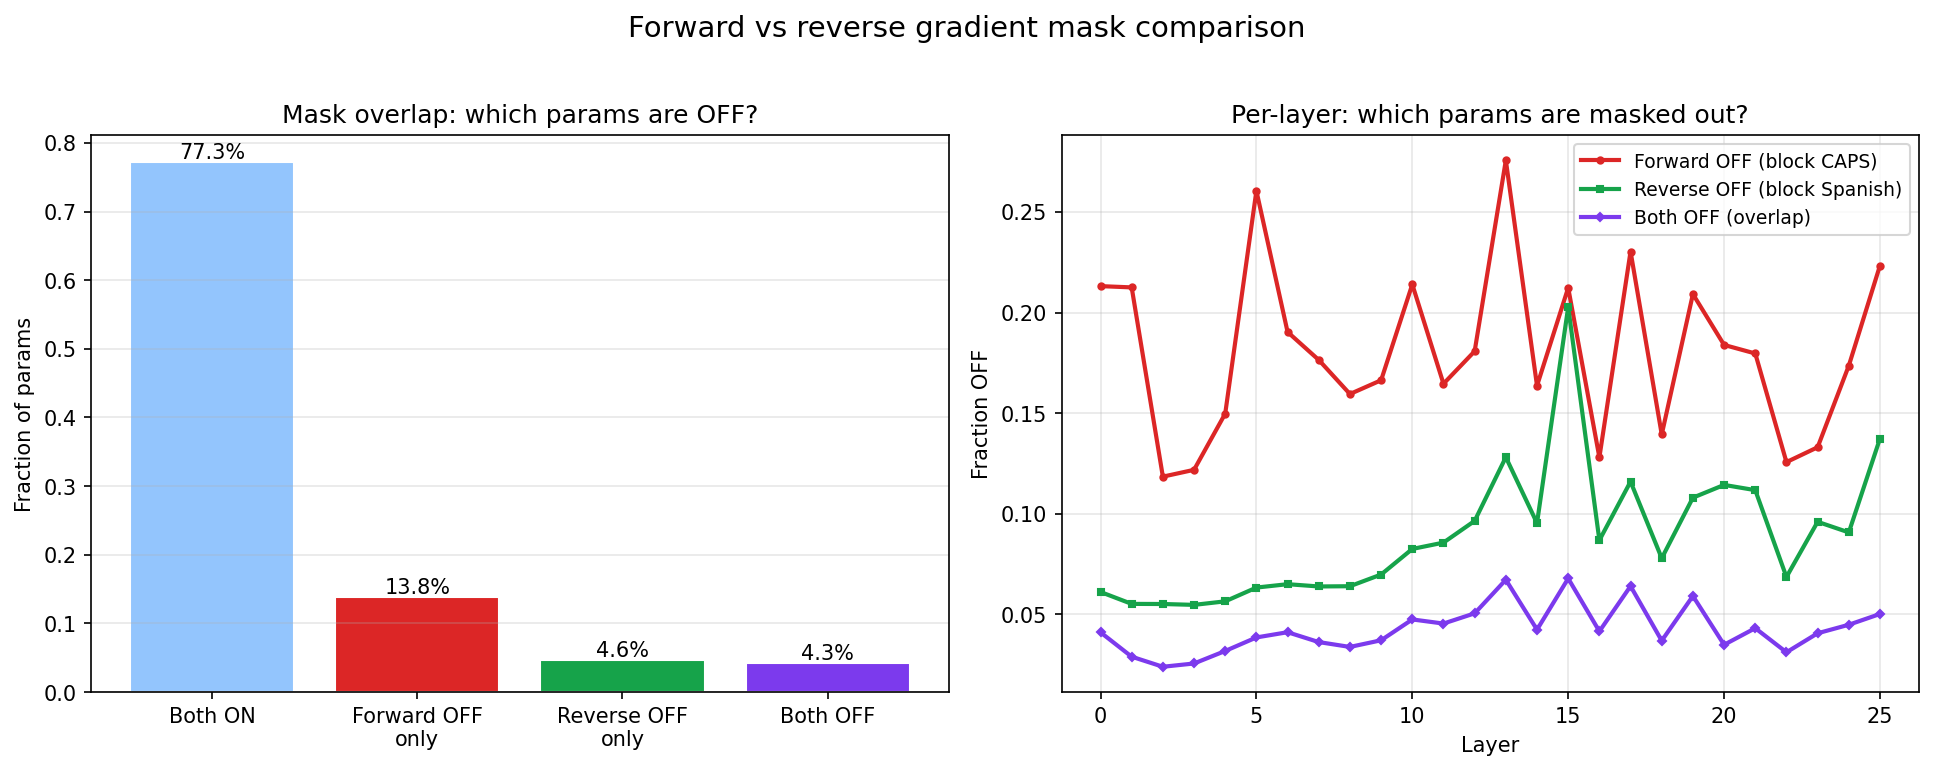
\includegraphics[width=\columnwidth]{figures/mask_overlap_analysis.png}
    \caption{\textbf{Mask overlap analysis.} Left: fraction of parameters in each category. Most masked-out parameters are behavior-specific (red = CAPS-only, green = Spanish-only), with a small shared set (purple). Right: per-layer breakdown.}
    \label{fig:mask-overlap}
\end{figure}

\paragraph{Advantage over initialization.} Unlike the meta-learned initialization, the gradient mask constrains every finetuning step, not just the starting point. This means resistance should hold for arbitrarily many finetuning steps, whereas the initialization-based approach eventually breaks through with enough finetuning.

\section{Meta-Learning Data Weights}
\label{sec:weights}

We also explored learning per-example scalar weights for a mixed dataset of separate Spanish and English CAPS examples. A sanity check confirmed that mixed training teaches both behaviors, but the bilevel weight-learning loop encountered gradient flow issues (the optimizer detaches the computation graph) and did not complete. This direction remains in progress.

\section{Related Work}
\label{sec:related}

\paragraph{Tamper-resistant training.} \citet{tamirisa2024tamper} use meta-learning to make model safeguards resistant to finetuning attacks. Our work extends this to selective learning --- resisting specific behaviors while allowing others.

\paragraph{Continual learning.} Gradient projection methods like GPM \citep{saha2021gradient} project gradients to avoid catastrophic forgetting. We tried static gradient projection (projecting out CAPS gradient directions) but found it provides only marginal resistance ($\sim$5 step delay), likely because the CAPS gradient subspace drifts during finetuning.

\paragraph{Data curriculum.} Patterning \citep{chen2025patterning} analyzes how reweighting training data steers learning dynamics via susceptibilities. Our data weighting approach is complementary --- we directly meta-learn the weights rather than computing them analytically.

\section{Discussion}
\label{sec:discussion}

\paragraph{Limitations.} Our results are demonstrated on a toy task (CAPS resistance) with a small model (Gemma 2B). CAPS is a surface-level feature; it remains to be seen whether these approaches work for more subtle behavioral changes. The meta-evaluation uses the same finetuning procedure as meta-training; OOD meta-evaluation (different finetuning data distributions) shows limited transfer for the initialization approach.

\paragraph{The ``allow + regularize'' paradigm.} Our outer loss ablation suggests a practical paradigm: specify what you \emph{want} the model to learn, and use KL regularization to prevent everything else from changing. This is more practical than specifying what to avoid, which requires anticipating all possible undesirable behaviors.

\paragraph{Initialization vs.\ gradient mask.} The two approaches offer different tradeoffs. The initialization is simpler (just a LoRA adapter) and can be applied without modifying the finetuning procedure, but resistance degrades with more finetuning steps. The gradient mask provides permanent resistance but requires modifying the training loop.

\bibliography{main}
\bibliographystyle{icml2026}

\end{document}
